\section{Is Platt scaling calibrated?}
\label{sec:challenges-measuring}

In this section, we show why methods like Platt scaling and temperature scaling are (i) less calibrated than reported and (ii) it is difficult to tell how miscalibrated they are. The issue is that it is very difficult to measure the calibration error of models that output a continuous range of values. We show, both theoretically and with experiments on CIFAR-10 and ImageNet, why the calibration error of such models is \emph{underestimated}.
We defer proofs to Appendix~\ref{sec:appendix-platt-not-calibrated}.

The key to estimating the calibration error is estimating the conditional expectation $\expect[Y \mid f(X)]$ where $f(X)$ is a continuous value; without smoothness assumptions on $\expect[Y \mid f(X)]$ (that cannot be verified in practice), this is impossible. This is analogous to the difficulty of measuring the mutual information between two continuous signals~\cite{paninski2003entropy}.

To approximate the $\ell_p$ calibration error, prior work bins the output of $f$ into $B$ intervals.
The calibration error in each bin is estimated as the difference between the average value of $f(X)$ and $Y$ in that bin.
Note that the binning here is for evaluation only, whereas in histogram binning is used for the recalibration method itself.
We formalize the notion of this binned calibration error below.

% \ak{Is the above text enough to motivate these definitions, or should I add more text?}
% \begin{definition}
% A binning scheme $\mathcal{B}$ is a set of $B$ disjoint intervals $I_1, \cdots, I_B$ that cover $[0, 1]$.
% \end{definition}

\begin{definition}
The binned version of $f$ outputs the average value of $f$ in each bin $I_j$:
\begin{align}
f_{\mathcal{B}}(x) = E[f(X) \mid f(X) \in I_j] \quad\quad\quad \mbox{where }x \in I_j
\end{align} 
\end{definition}
\pl{hoping you could just reuse the binning definition from setup, so you just have to write $\hat f$, or better $\bar f$ or $f_\text{binned}$ or some macro}

Given $\bins{}$, the binned calibration error of $f$ is simply $\lpce(f_{\bins{}})$.
A simple example shows that using binning to estimate the $\ell_p$ calibration error can severely underestimate the true $\ell_p$ calibration error, even for $p=1$, the average calibration error.

\newcommand{\continuousNotCalibratedText}{
For any binning scheme $\bins{}$, $p \in \mathbb{Z}^+$, and continuous bijective function $f : [0, 1] \to [0, 1]$, there exists a distribution $P$ over $X, Y$ s.t. $\lpce(f_{\bins{}}) = 0$ but $\lpce(f) \geq 0.49$.
Note that for all $f$, $0 \leq \lpce(f) \leq 1$.
}

\begin{example}
\label{ex:continuous-not-calibrated}
\continuousNotCalibratedText{}
\end{example}

\newtheorem*{continuousNotCalibrated}{Restatement of Example~\ref{ex:continuous-not-calibrated}}

The intuition is that in each interval $I_j$ in $\bins{}$, the model could underestimate the true probability $\expect[Y \mid f(X)]$ half the time, and overestimate the probability half the time. So if we average over the entire bin the model appears to be calibrated, even though it is very uncalibrated. The formal construction is in Appendix~\ref{sec:appendix-platt-not-calibrated}.

Next, we show that given a function $f$, its binned version always has lower calibration error. The proof, in Appendix~\ref{sec:appendix-platt-not-calibrated}, is by Jensen's inequality. Intuitively, averaging a model's prediction within a bin allows errors at different parts of the bin to cancel out with each other. This result is similar to Theorem 2 in recent work~\cite{vaicenavicius2019calibration}.

\newcommand{\binningLowerBoundText}{
Given binning scheme $\bins{}$ and model $f : \mathcal{X} \to [0, 1]$, we have:
\[  \lpce(f_{\bins{}}) \leq \lpce(f) \]
}

\begin{proposition}[Binning underestimates error]
\label{prop:bin_low_bound}
\binningLowerBoundText{}
\end{proposition}

\newtheorem*{binningLowerBound}{Restatement of Proposition~\ref{prop:bin_low_bound}}

\subsection{Experiments}

Our experiments on ImageNet and CIFAR-10 suggest that previous work reports numbers which are lower than the actual calibration error of their models. Recall that binning lower bounds the calibration error. We cannot compute the actual calibration error but if we use a `finer' set of bins then we get a tighter lower bound on the calibration error.

As in~\cite{guo2017calibration}, our model's objective was to output the top predicted class and a confidence score associated with the prediction. For ImageNet, we started with a trained VGG16 model with an accuracy of 64.3\%. We split the validation set into 3 sets of size $(20000, 5000, 25000)$. We used the first set of data to recalibrate the model using Platt scaling, the second to select the binning scheme $\mathcal{B}$ so that each bin contains an equal number of points, and the third to measure the binned calibration error. We calculated $90\%$ confidence intervals for the binned calibration error using 1,000 bootstrap resamples and performed the same experiment with varying numbers of bins.
% from the TensorFlow Keras library

Figure~\ref{fig:imagenet_lower_bound} shows that as we increase the number of bins on ImageNet, the measured calibration error is higher and this is statistically significant. For example, if we use 15 bins as in~\cite{guo2017calibration}, we would think the $\ell_2$ calibration error is around 0.02 when the calibration error is at least twice as high. Figure~\ref{fig:cifar_10_lower_bound} shows similar findings for CIFAR-10, and in Appendix~\ref{sec:appendix_platt_experiments} we show that our findings hold even if we use $\ell_1$ calibration error and alternative binning strategies.

\begin{figure}
     \centering
     \begin{subfigure}[b]{0.4\textwidth}
         \centering
         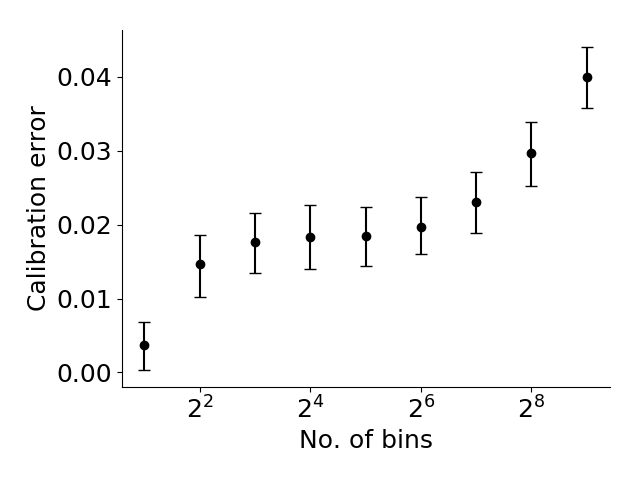
\includegraphics[width=\textwidth]{l2_lower_bound_imagenet_plot}
         \caption{ImageNet.}
         \label{fig:imagenet_lower_bound}
     \end{subfigure}
     \hfill
     \begin{subfigure}[b]{0.4\textwidth}
         \centering
         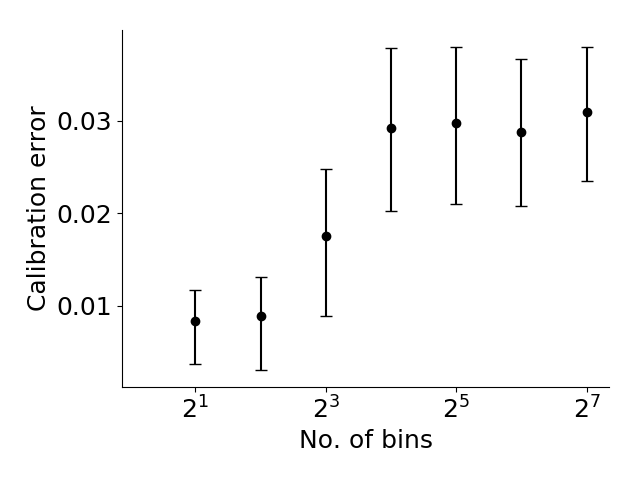
\includegraphics[width=\textwidth]{l2_lower_bound_cifar_plot}
         \caption{CIFAR-10.}
         \label{fig:cifar_10_lower_bound}
     \end{subfigure}
        \caption{
        Binned $\ell_2$ calibration errors of a recalibrated VGG-net model on CIFAR-10 and ImageNet with $90\%$ confidence intervals. The binned calibration error increases as we increase the number of bins. This suggests that binning cannot be reliably used to measure the true calibration error.
        }
        \label{fig:lower_bounds}
\end{figure}


% We might also wish to compare the calibration of different candidate models.

% \footnote{One possibility is to modify the calibration metric, for example to only require our model to be calibrated for all possible intervals of width $\geq \epsilon$.}

% One possibility is to modify the calibration metric, for example to only require our model to be calibrated for all possible intervals of width $\geq \epsilon$. 
% % This makes it difficult to ascertain if a model has a desired calibration error, or which of two models is better calibrated.

% We see three potential ways to resolve this:
% \begin{enumerate}
% \item Add a smoothness constraint on $E[Y | f(X)$], for example assume $E[Y | f(X)]$ is $L$-Lipschitz. Smoothness assumptions are common when training a model, but it is unsatisfying to assume a value of $L$, which we do not know, when \emph{evaluating} a model.
% \item Explore alternative metrics for calibration. For example, perhaps we only require our model to be calibrated for all possible intervals of width $\geq \epsilon$. 
% \item Discretize the outputs of the final model, so that it only outputs a finite number of values.
% \end{enumerate}

% In this paper we explore (3), but (1) and (2) are good directions for future research.

